
%\chapter{Methode} % Main chapter title
%\label{chapter3:Methode} % Change X to a consecutive number; for referencing this chapter elsewhere, use \ref{ChapterX}


%-----------------------------------
% SUBSECTION "Sniffer"
%-----------------------------------

\section{Sniffer Device}
% \textcolor{red}{Was ist ein Sniffer}\\
% Ein Sniffer ist grundsätzlich ein Gerät oder ein Software-Tool welches die Kommunikation zweier oder mehrerer Geräten überwachen und aufzeichnen kann.

% Ein solcher Sniffer wird Beispielsweise oft eingesetzt um den Netzwerkverkehr zu überwachen. Ein bekanntes Beispiel eines Sniffers dieser Art ist die Sniffer-Software Wireshark.\\

% Der Sniffer wie er auch in dieser Projektarbeit entwickelt wird, ist Physisch und wird direkt an einen Datenbus gehängt um von diesem lesen zu können.
% Dabei fängt der Sniffer die versendeten Datenpakete auf dem Bus ab ohne jegliche Störungen oder
% Einschränkungen der Kommunikation der Geräte zu verursachen.

Ein Sniffer ist ein Gerät oder Software-Tool, das in der Lage ist, die Kommunikation zwischen zwei oder mehreren Geräten zu überwachen und aufzuzeichnen. Diese Art von Werkzeug wird häufig verwendet um den Datenverkehr in Netzwerken oder auf Kommunikationsbussen zu analysieren.

Ein bekanntes Beispiel für ein solches Sniffer-Tool ist die Software Wireshark, die weit verbreitet zur Überwachung von Netzwerkprotokollen eingesetzt wird.

Im Rahmen dieser Projektarbeit wird ein physischer Sniffer entwickelt, der direkt an einen Datenbus angeschlossen wird, um die auf dem Bus übertragenen Datenpakete zu lesen. Dabei agiert der Sniffer passiv und erfasst die übertragenen Daten ohne die Kommunikation zwischen den Geräten zu beeinflussen
oder zu stören.

%--------------------------------------------------------------------------------
% SECTION Stand von Konkurenzprodukten
%--------------------------------------------------------------------------------

\section{Recherche bestehende Produkte}
\label{sec:recherche}

In einer Recherche zu bereits auf dem Markt vorhandenen MVB-Sniffern wurden verschiedene Varianten
gefunden. Teilweise wurden Anforderungen, die an den zu entwickelten Sniffer gestellt wurden, erfüllt.
Es wurden drei Geräte gefunden welche in diesem Kapitel etwas näher vorgestellt werden. In den folgenden Abschnitten sind dazu die verschiedenen Geräte mit dessen Merkmalen aufgelistet. Abschliessend wird in diesem Unterkapitel darauf eingegangen was den Sniffer, welcher entwickelt werden soll, ausmacht und welchen Vorteil dieser in der künftigen Anwendung bringen soll.

%\textbf{Sniffer 1: AMiT MVB Analyzer RB-MVB/AN01}\\[2ex]
\begin{minipage}{0.4\textwidth}
  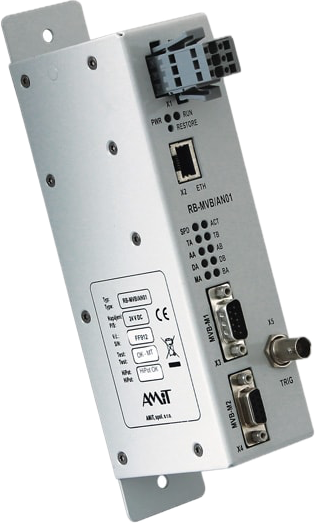
\includegraphics[width=0.7\linewidth]{Figures/Chap3/Konkurenz/Amit.png}
  \captionof{figure}{\mbox{AMiT MVB Analyzer \cite{Amit}}}
  \label{fig:AmitAnalyzer}
\end{minipage}
\hfill
\begin{minipage}{0.57\textwidth}
  \begin{tabular}{|m{3.3cm}|m{4.2cm}|}
  \hline
    \multicolumn{2}{|c|}{\textbf{AMiT MVB Analyzer RB-MVB/AN01}} \\ \hline
    \textbf{Firma} & AMiT Transportation \\ \hline
    \textbf{Datenbus} & MVB (EMD/ESD Kapitel \ref{Übertragungsmedien}) \\ \hline
    \textbf{Datenraten} & MVB: 1,5 Mbps / Ethernet: 10/100 Mbps \\ \hline
    \textbf{Galvanische \mbox{Trennung}} & nur Ethernet \\ \hline
    \textbf{Schnittstellen} & MVB: D-Sub 9 Pol / Ethernet: RJ45 \\ \hline
    \textbf{Stromversorgung} & 16.8–33.6 V DC \\ \hline
    \textbf{Einsatztemperatur} & -40 °C bis 70 °C \\ \hline
    \textbf{Schutzart} & IP20 \\ \hline
    \textbf{Gewicht} & 0.9 kg \\ \hline
    \textbf{Abmessungen} & 33 × 228 × 87 mm \\ \hline
    \textbf{Software} & Wireshark-Plug-in \\ \hline
    \textbf{Besonderheiten} & Redundantes MVB Interface (A und B Kapitel \ref{Übertragungsmedien}) \\ \hline
  \end{tabular}

\end{minipage}

%\textbf{Sniffer 2: Ci4Rail ModuSio MIO03 MVB/CAN Sniffer}\\[2ex]
\begin{minipage}{0.4\textwidth}
  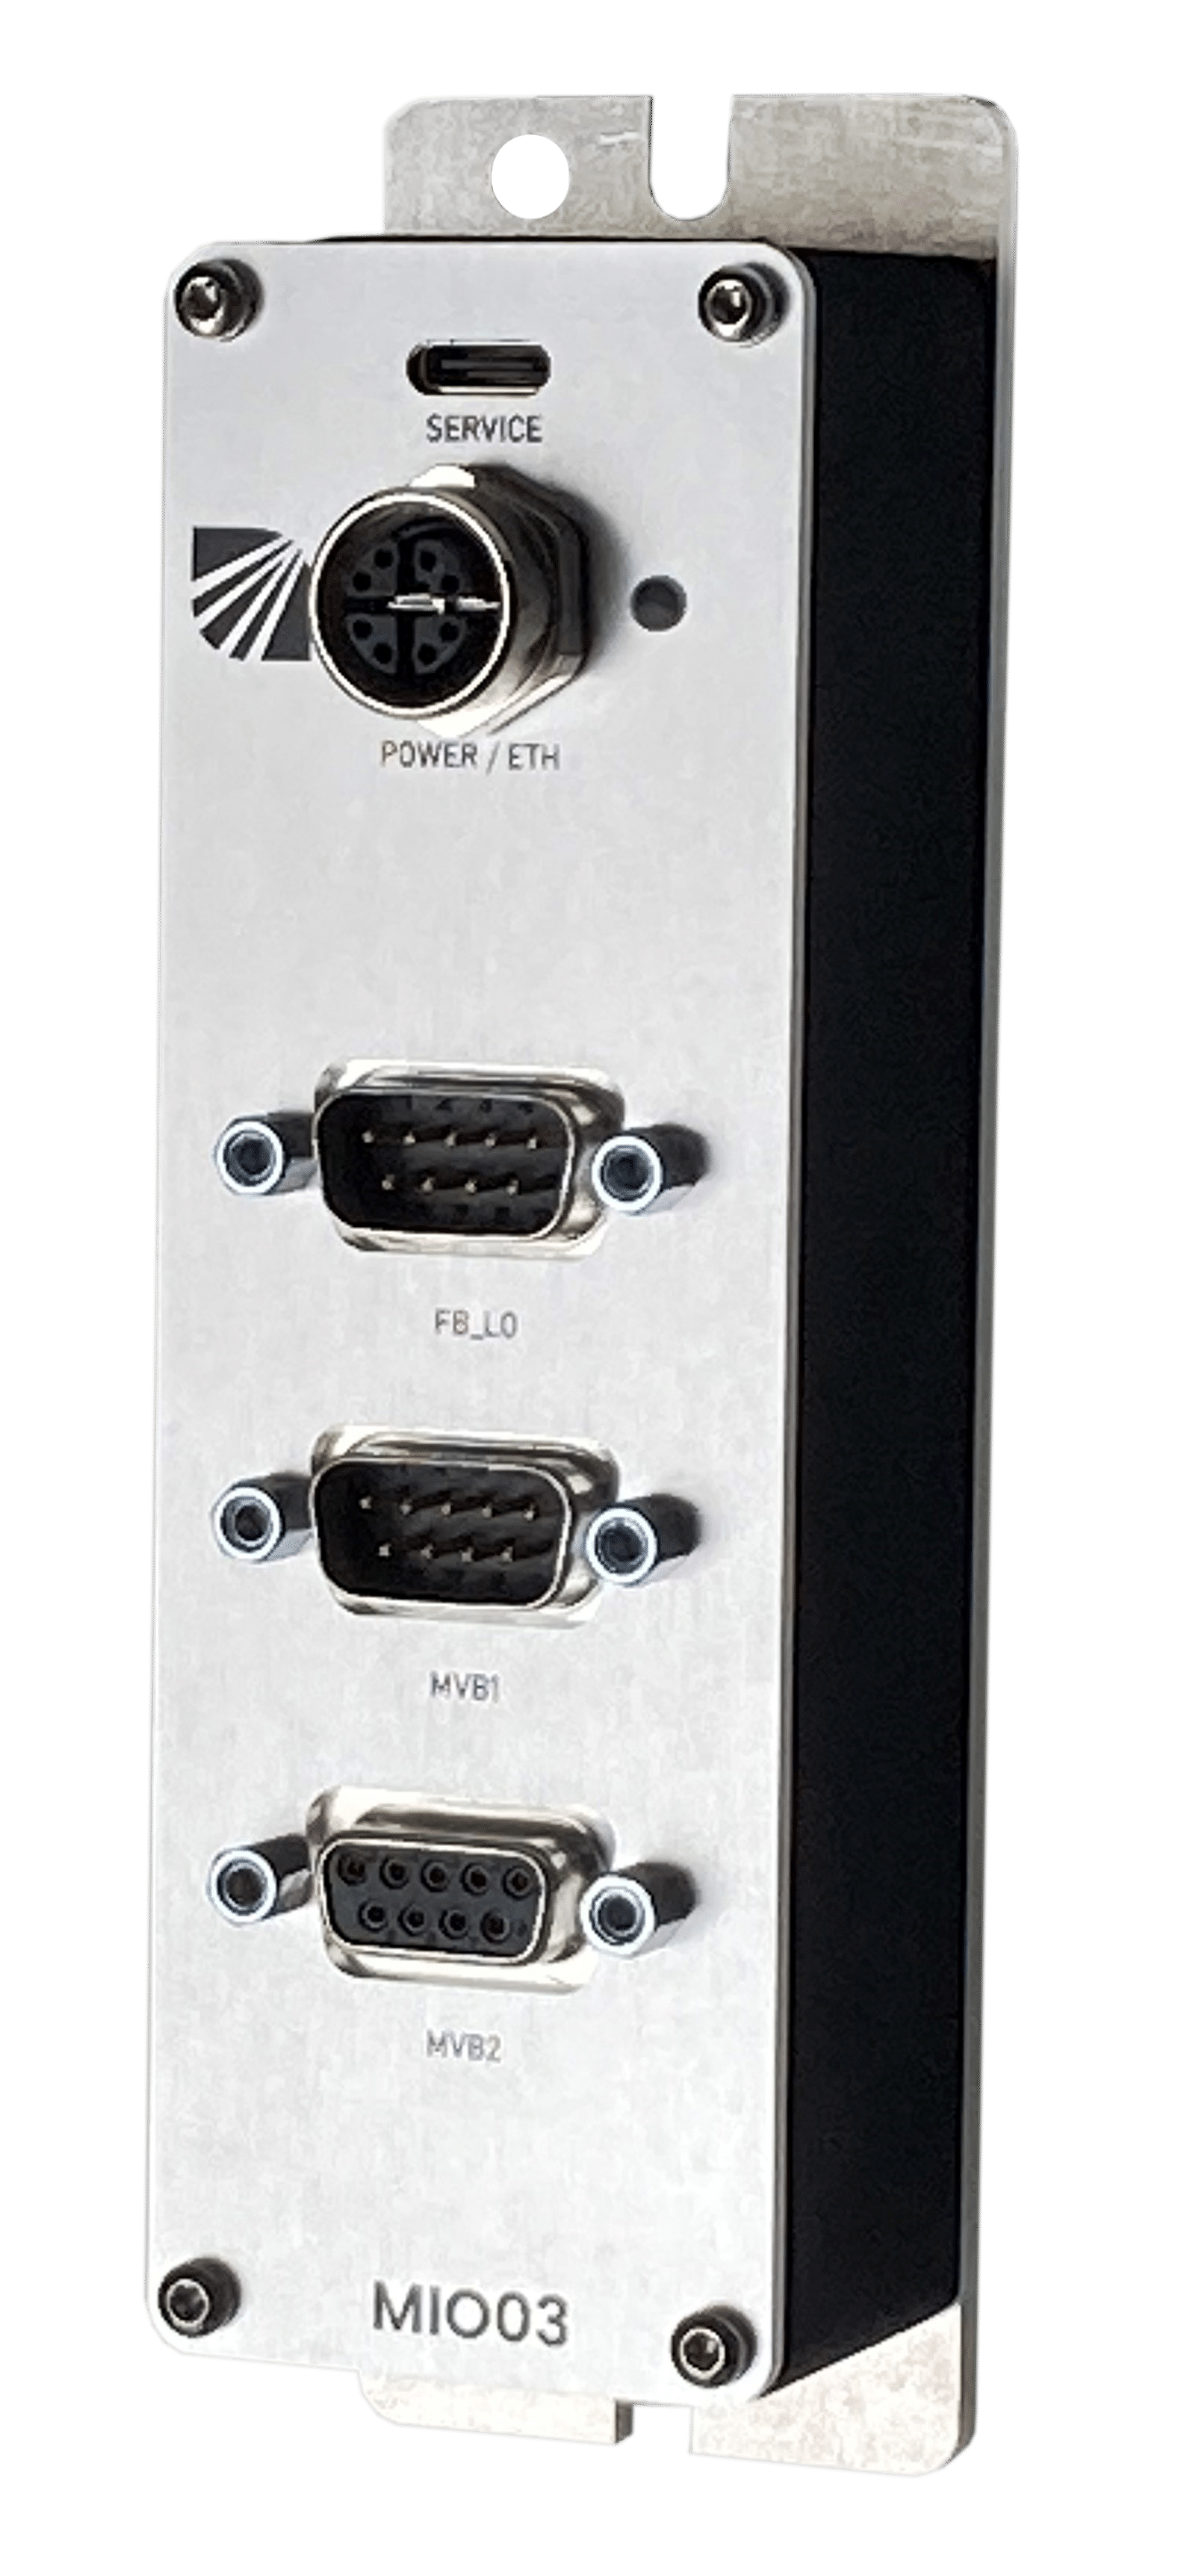
\includegraphics[width=0.7\linewidth]{Figures/Chap3/Konkurenz/CI4Rail.png}
  \captionof{figure}{\mbox{Ci4Rail Sniffer \cite{Ci4Rail}}}
  \label{fig:Ci4RailSniffer}
\end{minipage}
\vspace{0.3cm}
\hfill
\begin{minipage}{0.57\textwidth}
  \begin{tabular}{|m{3.3cm}|m{4.2cm}|}
   \hline
   \multicolumn{2}{|c|}{\textbf{Ci4Rail ModuSio MIO03 MVB/CAN Sniffer}} \\ \hline
    \textbf{Firma} & Ci4Rail \\ \hline
    \textbf{Datenbus} & MVB (EMD/ESD Kapitel \ref{Übertragungsmedien}), CAN \\ \hline
    \textbf{Datenraten} & MVB: 1,5 Mbps / CAN: bis zu 1 Mbps / Ethernet: 10/100 Mbps \\ \hline
    \textbf{Galvanische \mbox{Trennung}} & 750V DC (MVB/CAN/Shield) \\ \hline
    \textbf{Schnittstellen} & MVB: D-Sub 9 Pol, CAN: D-Sub 9 Pol , Ethernet: M12, Service: USB-C, WLAN: IEEE 802.11b/g/n  \\ \hline
    \textbf{Stromversorgung} & PoE oder 12/24 V DC \\ \hline
    \textbf{Einsatztemperatur} & -40 °C bis 70 °C \\ \hline
    \textbf{Schutzart} & keine Angabe \\ \hline
    \textbf{Gewicht} & keine Angabe \\ \hline
    \textbf{Abmessungen} & 151 × 42 × 51 mm \\ \hline
    \textbf{Software} &  Open Source APIs für SW-Integration \\ \hline
    \textbf{Besonderheiten} & WLAN-Firmwareupdates, CAN-Sniffer \\ \hline
  \end{tabular}
%\textcolor{red}{IP\ Based\ Sniffer}

\end{minipage}
\vspace{0.3cm}
%\newpage
%\textbf{Sniffer 3: Yacer MVB Protocol Analyzer}\\[2ex]
\begin{minipage}{0.4\textwidth}
  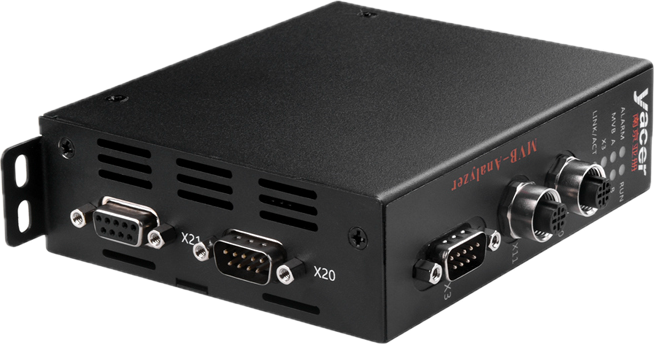
\includegraphics[width=1\linewidth]{Figures/Chap3/Konkurenz/Yacer.png}
  \captionof{figure}{MVB Protocol Analyzer \cite{Yacer}}
  \label{fig:YacerAnalyzer}
\end{minipage}
\hfill
\begin{minipage}{0.57\textwidth}
  \begin{tabular}{|m{3.3cm}|m{4.2cm}|}
    \hline
    \multicolumn{2}{|c|}{\textbf{Yacer MVB Protocol Analyzer}} \\ \hline
    \textbf{Firma} & Yacer \\ \hline
    \textbf{Datenbus} & MVB (EMD/ESD Kapitel \ref{Übertragungsmedien}), CAN \\ \hline
    \textbf{Datenraten} & MVB: 1,5 Mbps / CAN: bis zu 1 Mbps / Ethernet: 10/100 Mbps \\ \hline
    \textbf{Galvanische \mbox{Trennung}} & keine Angabe \\ \hline
    \textbf{Schnittstellen} & MVB: D-Sub 9 Pol, CAN: D-Sub 9 Pol , Ethernet: M12 \\ \hline
    \textbf{Stromversorgung} & 9–36 V DC (LV), 18–75 V DC (MV), \\ 
                                & 40–160 V DC (HV) \\ \hline
    \textbf{Einsatztemperatur} & -40 °C bis 70 °C \\ \hline
    \textbf{Schutzart} & keine Angabe \\ \hline
    \textbf{Gewicht} & 500 g \\ \hline
    \textbf{Abmessungen} & 124 × 36 × 104 mm \\ \hline
    \textbf{Software} & MVB-Monitor-Software \\ \hline
    \textbf{Besonderheiten} & Redundantes MVB Interface (A und B Kapitel \ref{Übertragungsmedien}), CAN-Sniffer \\ \hline
  \end{tabular}
\end{minipage}

Die Datenblätter von den Herstellern sind im Anhang \ref{app:File13}, \ref{app:File14} und \ref{app:File14} abgelegt.
%-----------------------------------
% SUBSECTION "Abgrenzung"
%-----------------------------------


\subsection{Angrenzung zu den bestehenden Produkten}

Der vorgestellte MVB-Sniffer weist im Vergleich zu bestehenden Produkten wie dem Yacer MVB-Analyzer, dem Ci4Rail MIO03 MVB/CAN Sniffer und dem AMiT MVB Analyzer mehrere technische und funktionale Unterschiede auf. Ein zentraler Unterschied liegt in der Integration von BLE (Bluetooth Low Energy), die eine kabellose Datenübertragung ermöglicht und somit die Verbindung zu mobilen Geräten oder PCs vereinfacht. Dadurch kann der Sniffer einfach mit mobilen Geräten oder PC verbunden werden, was eine zusätzliche Verkabelung überflüssig macht und die Handhabung erleichtert.

Ein weiterer Unterschied liegt in der Datenfilterung, die eine Selektion relevanter MVB-Daten gewährleistet. Dies reduziert die zu analysierende Datenmenge und kann die Effizienz bei der Fehlersuche und Diagnose in Netzwerken mit hohem Datenverkehr verbessern.

Auch in Bezug auf die Bedienung gibt es Unterschiede. Im Gegensatz zu einigen Konkurrenzprodukten soll der MVB-Sniffer ohne zusätzliche Software auskommen. In Zukunft soll der Sniffer über eine Web App konfiguriert werden können sowie Daten Visualisiert werden können

Im Bereich der Hardware soll der Sniffer durch seine kompakte Bauweise und sein geringes Gewicht in Zukunft hervorstechen. Diese Eigenschaften könnten die Mobilität und den Transport erleichtern. Ein integrierter Akku ermöglicht zudem den Einsatz des Sniffers in Situationen, in denen keine externe Stromversorgung verfügbar oder in der Nähe ist.

Zusammenfassend weist der MVB-Sniffer im Vergleich zu bestehenden Lösungen wie dem Yacer MVB-Analyzer, dem Ci4Rail MIO03 und dem AMiT MVB Analyzer Besonderheiten wie die BLE-Funktion, eine einfache Bedienbarkeit, den Verzicht auf Zusatzsoftware, einen integrierten Akku sowie eine kompakte Bauweise auf.